\documentclass{article} % Dokumentklasse: Artikel, geeignet für Berichte oder Ausarbeitungen
\usepackage{graphicx} % Ermöglicht das Einfügen von Bildern mit \includegraphics

\title{circuitikz} % Titel des Dokuments
\author{Luzin Timofey, David Kammerstetter, Florian Kastenauer, Felix Sator} % Autorenangabe
\date{20.10.2025} % Datum

\usepackage{circuitikz} % Wichtiges Paket: erlaubt das Zeichnen elektrischer Schaltungen in LaTeX

\begin{document}

\maketitle % Erstellt Titelseite mit Titel, Autor und Datum

\newpage % Neue Seite nach Titelseite


\section{Einleitung} % Abschnitt: Einführung

% Kurze Beschreibung, was circuitikz ist und wofür es verwendet wird
Circuitikz ist ein LaTeX-Paket welches verwendet wird, um elektrische und elektronische Schaltpläne direkt in LaTeX zu zeichnen. Es stellt eine Sammlung von Symbolen und Befehlen bereit, um Widerstände, Kondensatoren, Transistoren, Spannungsquellen usw. einfach zu zeichnen.

\subsection{Package}
% Erklärung, wie das Paket eingebunden wird
Um das circuitikz-Paket in LaTeX zu verwenden, muss es zuerst importiert werden.
Das geschieht im Vorspann, vor \\begin{document} des LaTeX-Dokuments mit der Zeile: \\usepackage{circuitikz}.

\section{Schaltungen zeichnen}

\subsection{TikZ}
% circuitikz basiert auf TikZ – wichtig für das Verständnis der Syntax
circuitikz basiert auf TikZ, einem weiteren LaTeX-Paket, das sich mit dem Zeichnen von Grafiken befasst. Um circuitikz besser zu verstehen, sollte man sich zunächst mit TikZ vertraut machen, da einige Funktionen und Befehle auf die gleiche Weise verwendet werden.

\subsection{Linie}
% Grundelement: Linien verbinden Schaltungselemente
In circuitikz beginnt man immer mit einer Linie, weil alle Schaltungselemente an Liniensegmenten zwischen zwei Punkten platziert werden. Diese kann entwerder mit der Zeile \\draw (0,0) -- (2,0); oder mit \\draw (0,0) to (2,0); ausgefürt werden.

\begin{center}
\begin{circuitikz}
    \draw (0,0) -- (2,0); % Zeichnet eine einfache horizontale Linie
\end{circuitikz}
\end{center}

\subsection{Schaltungselemente}
% Beispiel: Widerstand zwischen zwei Punkten
Um ein Schaltungselement einzufügen und mit einer Linie zu verbinden, muss man die Zeile einfach zu \\draw (0,0) to[resistor] (2,0); ändern.

\begin{center}
\begin{circuitikz}
    \draw (0,0) to[resistor] (2,0); % Fügt einen Widerstand ein
\end{circuitikz}
\end{center}

% Hinweis: Viele Bauteile lassen sich direkt mit einem Schlüsselwort verwenden
Viele elektrische Schaltungselemente könne, so wie der Widerstand, einfach mit einem Wort eingefügt werden.

\subsubsection{Monopole}
% Monopole = Bauteile mit nur einem Anschluss (z. B. Ground)

\newcommand{\thiscirc}[1]{%
\texttt{#1}\kern5pt\hfill
\begin{circuitikz}%
\draw (0,0) node[ #1 ] {}; % Zeichnet Symbol als einzelnes Node
\end{circuitikz}%
{\hspace{5mm}}%
}

% Tabelle mit verschiedenen Monopolen
\renewcommand{\arraystretch}{2}
\begin{center}
\begin{tabular}{lll} 
\thiscirc{ground} & \thiscirc{sground} & \thiscirc{nground}\\
\thiscirc{rground} & \thiscirc{pground} & \thiscirc{cground}\\
\thiscirc{tlinestub} & \thiscirc{antenna} & \thiscirc{rxantenna}\\
\end{tabular}
\end{center}

% Erklärung: Monopole werden mit "node" platziert
Ein Monopol kann nur dann eingefügt werden wenn man den befehl "node", dann den namen des Monopls und dann erst die zweite Koordinate einfügt. z.B. \\draw (0,0) node[ground]{} to (0,0); 

\begin{center}
\begin{circuitikz}
  \draw (0,0) node[ground]{} to (0,0); % Ground-Symbol an Position (0,0)
\end{circuitikz}
\end{center}

% Einfacher Stromkreis mit Ground, Spannungsquelle und Widerstand
\begin{center}
\begin{circuitikz}
  \draw (0,0) node[ground]{} to (0,0); 
  \draw (0,0) to[V, l=$U$] (0,3);
  \draw (0,3) to[R, l=$R$] (3,3);
  \draw (3,3) to (3,0);
  \draw (3,0) to (0,0);
\end{circuitikz}
\end{center}

\subsubsection{Bipole}
% Bipole: Bauteile mit zwei Anschlüssen (z. B. Widerstände, Dioden, Spulen)

\newcommand{\bipole}[1]{%
\texttt{#1}\kern5pt \hfill
\begin{circuitikz}%
\draw (0,0) to[ #1 ] (2,0); % Zeichnet Bipol zwischen zwei Punkten
\end{circuitikz}%
\hspace{5mm}%
}

% Übersicht gängiger Bipole
\renewcommand{\arraystretch}{3}
\begin{center}
\begin{tabular}{ll} 
\bipole{ammeter} & \bipole{voltmeter} \\
\bipole{short} & \bipole{open} \\
\bipole{lamp} & \bipole{generic} \\
\bipole{tgeneric} & \bipole{ageneric} \\
\bipole{fullgeneric} & \bipole{tfullgeneric} \\
\bipole{memristor} & \bipole{american resistor} \\
\bipole{vR} & \bipole{american potentiometer} \\
\bipole{european resistor} & \bipole{european potentiometer} \\
\bipole{varistor} & \bipole{photoresistor} \\
\bipole{thermocouple} & \bipole{thermistor} \\
\bipole{thermistor ntc} & \bipole{fuse} \\
\bipole{afuse} & \bipole{battery} \\
\bipole{battery1} & \bipole{european voltage source} \\
\bipole{american voltage source} & \bipole{european current source} \\
\bipole{american current source} &  \\
\end{tabular}
\end{center}

\subsubsection{Dioden}
% Neue Tabelle: verschiedene Diodentypen
\newcommand{\bipole}[1]{%
\texttt{#1}\kern5pt \hfill
\begin{circuitikz}%
\draw (0,0) to[ #1 ] (2,0); 
\end{circuitikz}%
\hspace{5mm}%
}

\renewcommand{\arraystretch}{3}
\begin{center}
\begin{tabular}{ll} 
\bipole{empty diode} & \bipole{empty Schottky diode} \\
\bipole{empty Zener diode} & \bipole{empty tunnel diode} \\
\bipole{photodiode} & \bipole{empty diode} \\
\bipole{empty varcap} & \bipole{full diode} \\
\bipole{full Schottky diode} & \bipole{full Zener diode} \\
\bipole{full tunnel diode} & \bipole{full photodiode} \\
\bipole{full led} & \bipole{full varcap} \\
\bipole{squid} & \bipole{barrier} \\
\end{tabular}
\end{center}

\subsubsection{Dynamische Bipole}
% Tabelle mit dynamischen Bauteilen wie Kondensator, Spule, Quelle etc.
\newcommand{\bipole}[1]{%
\texttt{#1}\kern5pt \hfill
\begin{circuitikz}%
\draw (0,0) to[ #1 ] (2,0); 
\end{circuitikz}%
\hspace{5mm}%
}

\renewcommand{\arraystretch}{3}
\begin{center}
\begin{tabular}{ll} 
\bipole{capacitor} & \bipole{polar capacitor} \\
\bipole{variable capacitor} & \bipole{cute inductor} \\
\bipole{variable cute inductor} & \bipole{american inductor} \\
\bipole{variable american inductor} & \bipole{european inductor} \\
\bipole{variable european inductor} & \bipole{transmission line} \\
\bipole{vsourcesin} & \bipole{isourcesin} \\
\bipole{closing switch} & \bipole{opening switch} \\
\bipole{push button} & \\
\end{tabular}
\end{center}

% Hinweis auf Kurzformen von Symbolen
Für manche Bauteile gibt es auch abkürzungen. So wie V für Spannungsquelle oder R für Widerstand oder L für Spulen.

\subsection{Europäisch/Amerekanisch}
% Erklärung der Symbolstile: europäisch oder amerikanisch
In circuitikz kann man zwischen europäischen und amerikanischen Schaltsymbolen wählen. Dies kann man entweder dadurch steuern, dass man european oder american vor die Bezeichnung des Schaltelements schreibt, z.B. \\bipole{european resistor} oder \\bipole{american resistor} oder indem man den gesamten Schaltplan auf europäische oder amerikanische Symbole setzt. \\begin{circuitikz}[american] 

\begin{center}
\begin{circuitikz}[american] 
    \draw (0,0) to[resistor] (2,0); % Amerikanische Darstellung
\end{circuitikz}
\end{center}

\begin{center}
\begin{circuitikz}[european] 
    \draw (0,0) to[resistor] (2,0); % Europäische Darstellung
\end{circuitikz}
\end{center}

\subsection{Bezeichnung}
% Beschriftung von Bauteilen (Label)
Ein Schaltelement wird benannt, indem man die Zeile \\draw (0,0) to[resistor] (2,0); auf \\draw (0,0) to[resistor, l=$R$] (2,0); ändert. Damit wird ein Label (Beschriftung) R am Bauteil angezeigt.

\begin{center}
\begin{circuitikz}[european] 
    \draw (0,0) to[resistor, l=$R$] (2,0); % Label oberhalb
\end{circuitikz}
\end{center}

\begin{center}
\begin{circuitikz}[european] 
    \draw (0,0) to[resistor, l_=$R$] (2,0); % Label unterhalb
\end{circuitikz}
\end{center}

\subsection{Ströme/Spannungen}
% Darstellung von Strom- und Spannungspfeilen

\subsubsection{Ströme}
% Strompfeile (i=$i$)
Ströme werden mithilfe der Zeile \\draw (0,0) to[short, i=$i$] (2,0); dargestellt. 

\begin{center}
\begin{circuitikz}[european] 
    \draw (0,0) to[short, i=$i$] (2,0); % Strom von links nach rechts
\end{circuitikz}
\end{center}

\begin{center}
\begin{circuitikz}[european] 
    \draw (2,0) to[short, i_=$i$] (0,0); % Strom von rechts nach links
\end{circuitikz}
\end{center}

\subsubsection{Spannungen}
% Spannungspfeile (v^>=$U$)
Spannungen werden mithilfe der Zeile \\draw (0,0) to[open, vHoch>=$U$] (2,0); dargestellt.

\begin{center}
\begin{circuitikz}[european] 
    \draw (0,0) to[open, v^>=$U$] (2,0); % Spannung von links nach rechts
\end{circuitikz}
\end{center}

\begin{center}
\begin{circuitikz}[european] 
    \draw (2,0) to[open, v^>=$U$] (0,0); % Spannung von rechts nach links
\end{circuitikz}
\end{center}

\subsection{Schaltung}

\subsubsection{Leitungen}
% Beispiel für Leitungsverbindungen (Rahmen)
\begin{center}
\begin{circuitikz}[european] 
    \draw (0,0) to (6,0);
    \draw (6,0) to (6,4);
    \draw (6,4) to (0,4);
\end{circuitikz}
\end{center}

\subsubsection{Schaltungselemente}
% Beispielschaltung mit Spannungsquelle, Widerstand und Spule
\begin{center}
\begin{circuitikz}[european] 
    \draw (0,0) to (6,0);
    \draw (6,0) to[V, l=$U$] (6,4);
    \draw (6,4) to[R, l=$R$] (3,4);
    \draw (3,4) to[L, l=$L$] (0,4);
\end{circuitikz}
\end{center}

\subsubsection{Spannungen/Ströme}
% Erweiterte Schaltung mit Strom- und Spannungspfeilen
\begin{center}
\begin{circuitikz}[european] 
    \draw (0,0) to[short, *-] (6,0);
    \draw (6,0) to[V, l=$U$] (6,4);
    \draw (6,4) to[R, l=$R$] (3,4);
    \draw (3,4) to[L, l=$L$] (1,4);
    \draw (0,4) to[short, *-, i=$i$] (1,4);
    \draw (0,0) to[open, v^>=u] (0,4);
\end{circuitikz}
\end{center}

\section{Beispiel}
% Komplexeres Beispiel mit mehreren Strom- und Spannungspfaden
\begin{center}
\begin{circuitikz}[european]
\draw
  (0,0) to [short, *-] (6,0)
  to [V, l_=$\mathrm{j}{\omega}_m \underline{\psi}^s_R$] (6,2) 
  to [R, l_=$R_R$] (6,4) 
  to [short, i_=$\underline{i}^s_R$] (5,4) 
  (0,0) to [open, v^>=$\underline{u}^s_s$] (0,4) 
  to [short, *- ,i=$\underline{i}^s_s$] (1,4) 
  to [R, l=$R_s$] (3,4)
  to [L, l=$L_{\sigma}$] (5,4) 
  to [short, i_=$\underline{i}^s_M$] (5,3) 
  to [L, l_=$L_M$] (5,0); 
\end{circuitikz}
\end{center}

\section{Website}
% Hinweis auf die Online-Plattform circuit2tikz zur grafischen Erstellung von Schaltungen
Um das Erstellen von Schaltungen zu erleichtern, kann auch die Website
https://www.circuit2tikz.tf.fau.de/designer/ verwendet werden. Dort kann eine Schaltung – ähnlich wie in Programmen wie S-Plan oder E-Plan – per Drag-and-Drop erstellt werden. Anschließend lässt sich der erzeugte LaTeX-Code extrahieren und direkt in das eigene Dokument einfügen.

\subsection{Schaltung zeichnen}

% Screenshot des User Interface
\begin{center}
\begin{figure}[h]

\includegraphics[scale=0.4]{Bilder/website1.PNG}
\caption{User Interface}
\label{User Interface}
\end{figure} 
\end{center}

% Beispiel: TikZ-Schaltungscode aus der Website
\begin{center}
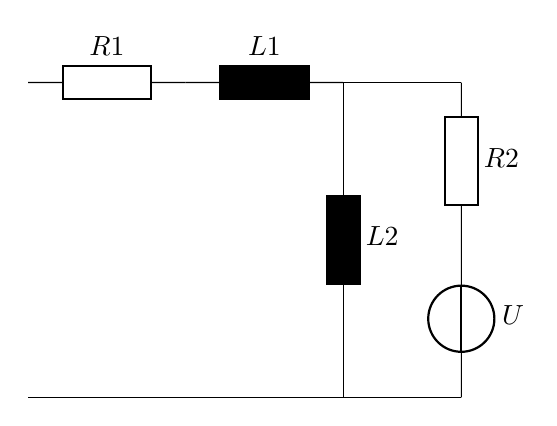
\begin{tikzpicture}
	% Pfade, Nodes und Verbindungen
	\draw (5.5, 5) to[european resistor, l={$R1$}] (7.5, 5); % Widerstand R1
	\draw (7.5, 5) to[european inductor, l={$L1$}] (9.5, 5); % Spule L1
	\draw (11, 5) to[european resistor, l={$R2$}] (11, 3); % Widerstand R2
	\draw (11, 3) to[european voltage source, l={$U$}] (11, 1); % Spannungsquelle U
	\draw (9.5, 5) to[european inductor, l={$L2$}] (9.5, 1); % Spule L2
	\draw (9.5, 5) -- (11, 5); % Verbindung oben
	\draw (11, 1) |- (5.5, 1); % Verbindung unten
\end{tikzpicture}
\end{center}

% Hinweis zum Abrufen des LaTeX-Codes von der Website
Auf den erzeugten LaTeX-Code kann durch einen Klick auf die Pfeile in der oberen rechten Ecke zugegriffen werden. Der Code muss nur kopiert und eingefügt werden.

% Screenshot: LaTeX-Code der Website
\begin{center}
\begin{figure}[h]

\includegraphics[scale=0.6]{Bilder/website 2.PNG} % Screenshot Code
\caption{LaTeX Code}
\label{LaTex Code}
\end{figure} 
\end{center}



\end{document}
